\section{Beschränktheits-Algorithmus}
\label{sec:algo}

\subsection{Beschränktheit des Erreichbarkeitsgraphen}
Wie in \cref{sec:struct} beschrieben, hält jedes Petri-Netz seinen eigenen
Erreichbarkeitsgraphen als Attribut. Beim Hinzufügen einer neuen Markierung in
den Erreichbarkeitsgraphen, wird geprüft, ob es eine Markierung auf dem Weg zur
Wurzel-Markierung gibt, die die m $\leftrightarrow$ m' Relation verletzt. Diese
Pfade werden mittels Breitensuche abgeschritten. Hierbei ist eine rückwärts
gerichtete Breitensuche mittelt der in einem \texttt{LinkedMarking} gehaltenen
\texttt{Edge}s zu den Vorgänger-Markierungen einfach implementierbar.

Sei \texttt{get\_predecessors} eine Methode um die Vorgänger-Knoten eines Knoten
in einem Erreichbarkeitsgraphen zu erhalten. Der \texttt{\textgreater}-Operator
führe für zwei Markierungen A und B den elementweisen Vergleich der Token-Anzahl
an jedem Index aus und gibt \texttt{true} zurück, wenn A an mindestens einer
Position eine größere Token-Anzahl als B enthält und an allen anderen Stellen
die Anzahl der Tokens gleich groß ist. %
Die Prüfung der m $\leftrightarrow$ m' Relation stellt
sich dann in Pseudocode wie folgt dar, wobei davon ausgegangen wird, dass die
Startmarkierung der Suche im Erreichbarkeitsgraphen vorhanden ist.

\begin{lstlisting}[language=python, morekeywords={do, algorithm, then}]
  algorithm check_bounded(r_graph, start_marking)
    visited_markings = Set() # of Markings
    visited_markings.add(start_marking)
    queue = DoubleEndedQueue()
    start_node = r_graph.get_node(start_marking)
    queue.append(start_node.get_predecessors())
    while not queue.is_empty() do
      other_node = queue.pop_first()
      if (visited_markings.contains(other)) then
        continue
      if (start_marking > other) then
        return false
      q.append(other.get_predecessors())
      visited_markings.add(other)
    return true
\end{lstlisting}

\subsection{Beschränktheit des Petri-Netzes}
Um die (Un)Beschränktheit eines Petri-Netzes festzustellen, werden bei der
Beschränktheitsanalyse so lang Transitionen geschaltet, bis entweder
\begin{itemize}
  \item alle möglichen Pfade durch das Petri-Netz beschritten wurden und keine
        aktiven Transitionen mehr vorhanden sind oder
  \item beim Aufbau des Erreichbarkeitsgraphen die Unbeschränktheit des Netzes
        festgestellt wurde.
\end{itemize}

Um alle möglichen Pfade in einem Petri-Netz zu beschreiten, wird in PetriCheck
eine Tiefensuche im Petri-Netz verwendet. Hierfür verfügt die Implementierung
des Petri-Netzes über eine Hilfsmethode, die eine Liste der gerade aktiven
Transitionen ausgeben kann:

\begin{lstlisting}[language=python, morekeywords={do, algorithm, then}]
  algorithm get_active_transitions(petri_net)
    output = []
    for transition in petri_net.transitions do
      if transition.is_active() then
        output.append(transition)
    return output
\end{lstlisting}

Im initialen Schritt des Algorithmus wird das Petri-Netz auf seine
Ausgangsmarkierung zurückgesetzt und der Erreichbarkeitsgraph reinitialisiert.
Hierbei werden alle bisherigen eventuell durch interaktives Schalten von
Transitionen vorhandenen Markierungen und Kanten gelöscht und nur der
Wurzelknoten, die Ausgangsmarkierung, hinzugefügt. Anschließend kann die rekursiv
formulierte Tiefensuche gestartet werden.

\begin{lstlisting}[language=python, morekeywords={do, algorithm, then}]
  algorithm is_bounded(petri_net)
    petri_net.reset()
    petri_net.r_graph.initialize()
    return is_bounded_rec(petri_net)
\end{lstlisting}

In der Tiefensuche wird zuerst die aktuelle Markierung gesichert, damit sie nach
dem Schalten einer Transition wiederhergestellt werden kann. Der rekursive
Abstieg erfolgt in der if-Bedingung, um beim Auffinden der ersten Verletzung der
m $\leftrightarrow$ m' Relation die Rekursion zu beenden. Der rekursive
Algorithmus lautet in Pseudocode:

\begin{lstlisting}[language=python, morekeywords={do, algorithm, then}]
  algorithm is_bounded_rec(petri_net)
    last_marking = petri_net.get_marking()
    for transition in get_active_transitions(petri_net) do
      # this call adds marking to r_graph and checks boundedness
      petri_net.trigger_transition(transition)
      if not petri_net.r_graph.is_bounded or not is_bounded_rec(petri_net) then
        return false
      petri_net.set_marking(last_marking)
    return true
\end{lstlisting}

Neben diesen Schritten wird in der Implementierung in PetriCheck noch der
aktuell beschrittene Pfad dokumentiert und zwei ggf. gefundene in m
$\leftrightarrow$ m' Relation stehende Markierungen für die Ausgabe gesichert.

Die Ansicht des Programms nach der Beschränktheitsanalyse der Beispieldatei 276 zeigt \cref{img:ex276_default}.

\begin{figure}[H]
  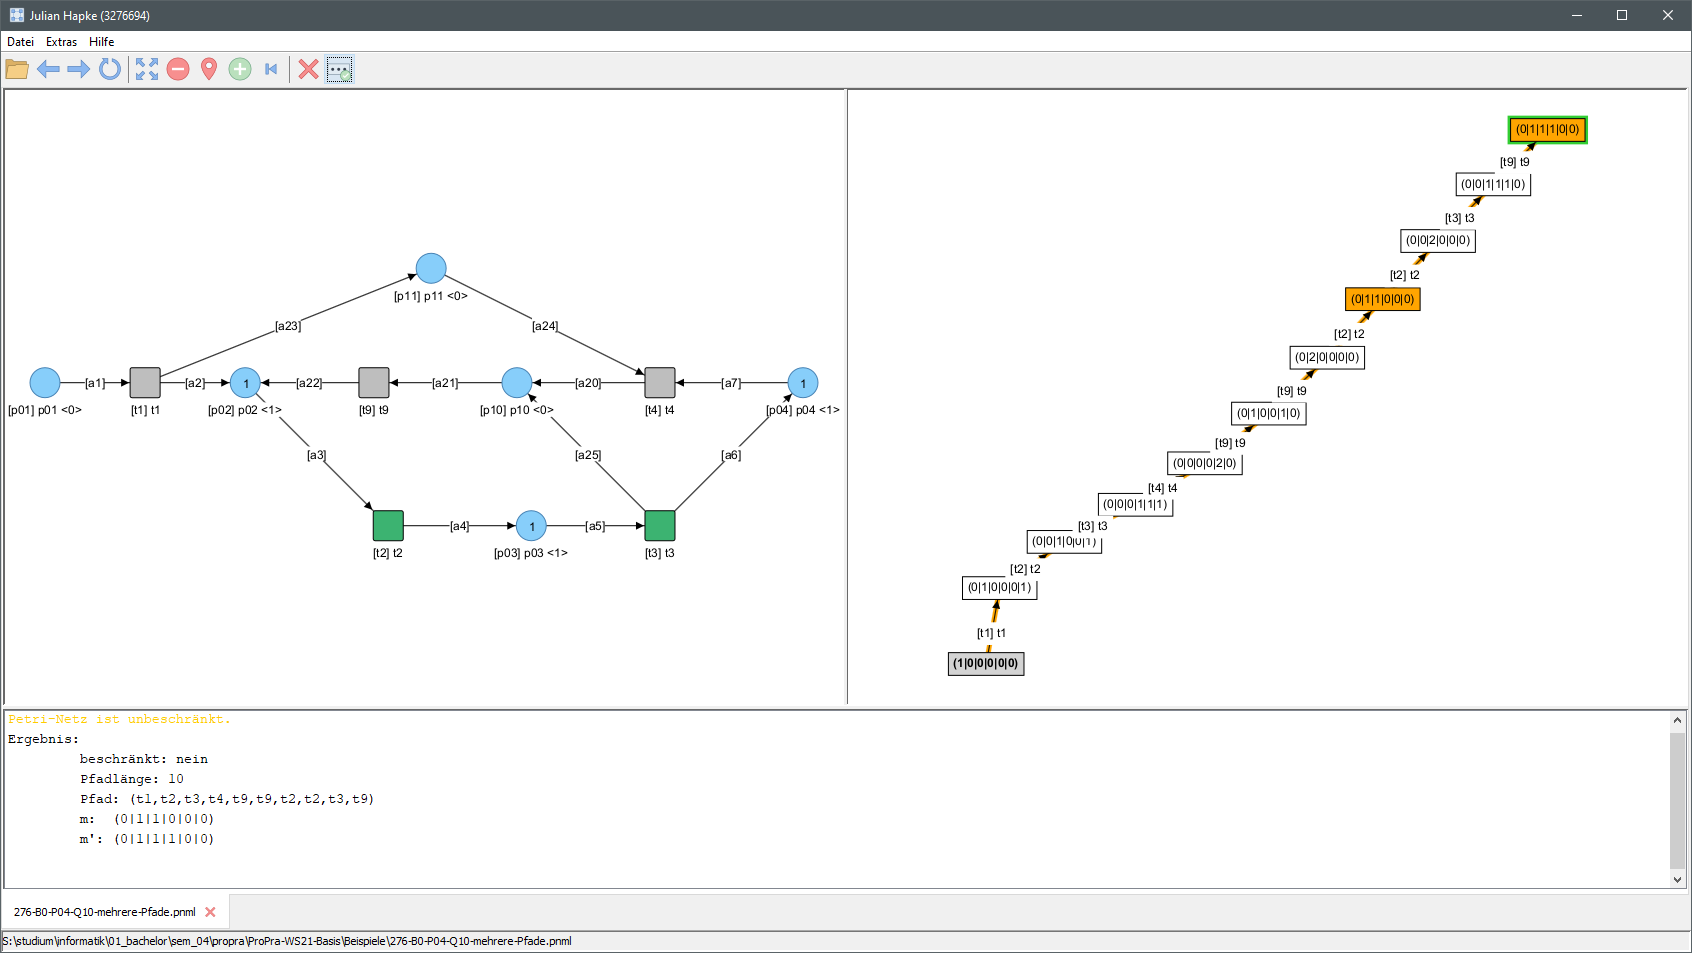
\includegraphics[width=\textwidth]{../img/Screenshot_276_default_layout.png}
  \caption{Beispieldatei 276 nach der Beschränktheitsanalyse}
  \label{img:ex276_default}
\end{figure}
